\chapter{8PSK \& Higher-Order PSK}
\label{ch:8psk}

\begin{nontechnical}
\textbf{8PSK is like using 8 different hand gestures instead of 4}---you can send 50\% more data per symbol, but the gestures are closer together, making them easier to confuse in noisy conditions.

\textbf{8PSK is like using 8 different hand gestures instead of 4}---you can send 50\% more data per symbol, but the gestures are closer together, making them easier to confuse in noisy conditions.

\textbf{The progression:}
\begin{itemize}
\item \textbf{BPSK:} 2 positions (up/down) = 1 bit/symbol
\item \textbf{QPSK:} 4 positions (corners) = 2 bits/symbol
\item \textbf{8PSK:} 8 positions (compass directions) = 3 bits/symbol $\leftarrow$ \emph{We are here}
\item \textbf{16-PSK:} 16 positions = 4 bits/symbol
\item \textbf{32-PSK:} 32 positions = 5 bits/symbol
\end{itemize}

\textbf{The trade-off:} More positions means faster data rate (8PSK is 1.5$\times$ faster than QPSK), but positions are closer together. This makes them easier to confuse when noise is present, requiring stronger signals (higher SNR) to work reliably.

\textbf{Real-world use:} \textbf{DVB-S2} satellite broadcasting uses 8PSK for HD channels because satellite bandwidth is expensive. The 50\% data rate increase translates to 50\% more channels in the same bandwidth. The trade-off is needing larger receiving dishes for adequate SNR.

\textbf{Why not go higher?} Beyond 8PSK, phase states become too closely spaced. Even tiny noise causes errors. For higher spectral efficiency, \textbf{QAM} (which varies both amplitude and phase) is more effective. This is why WiFi uses 64-QAM and 256-QAM, not 16-PSK or 32-PSK.

\textbf{Where you'll encounter 8PSK:}
\begin{itemize}
\item Satellite TV (DVB-S2 HD channels)
\item Military SATCOM (MILSTAR)
\item NASA deep-space missions (high-rate data return)
\item Microwave backhaul (cell tower point-to-point links)
\end{itemize}

\textbf{Angular spacing matters:}
\begin{itemize}
\item QPSK: 90° between positions (robust)
\item 8PSK: 45° between positions (moderate)
\item 16-PSK: 22.5° between positions (sensitive)
\end{itemize}
Smaller angular separation = easier to confuse = requires cleaner signal and better phase tracking.
\end{nontechnical}

\section{Overview}

\textbf{8-ary Phase-Shift Keying (8PSK)} encodes data using \textbf{8 equally-spaced phase states} positioned around the unit circle, transmitting \textbf{3 bits per symbol}. This provides 50\% higher spectral efficiency than QPSK at the cost of approximately 3.5~dB additional SNR requirement.

\begin{keyconcept}
8PSK achieves \textbf{3 bits/symbol} ($\sim$2.2~bps/Hz with pulse shaping), providing a middle ground between QPSK's robustness (2 bits/symbol) and 16-QAM's efficiency (4 bits/symbol). Its constant envelope property makes it ideal for satellite systems using nonlinear power amplifiers.
\end{keyconcept}

Higher-order PSK schemes ($M$-PSK) use $M$ phase states to transmit $\log_2(M)$ bits per symbol. However, beyond 8PSK, the reduced angular spacing between constellation points makes phase noise and additive noise increasingly problematic, leading to rapid BER degradation.

\section{Mathematical Description}

\subsection{8PSK Constellation}

The 8PSK constellation consists of 8 equally-spaced phase states positioned on a unit circle with angular separation of $45°$ ($\pi/4$ radians):

\begin{equation}
\phi_m = \frac{2\pi m}{8} = \frac{\pi m}{4}, \quad m = 0, 1, \ldots, 7
\end{equation}
where:
\begin{itemize}
\item $\phi_m$ = phase angle for symbol $m$ (radians)
\item $m$ = symbol index from 0 to 7
\end{itemize}

\subsection{Time-Domain Signal}

The transmitted signal for symbol $m$ is:
\begin{equation}
s_m(t) = A\cos(2\pi f_c t + \phi_m)
\end{equation}
where:
\begin{itemize}
\item $A$ = carrier amplitude
\item $f_c$ = carrier frequency (Hz)
\item $\phi_m$ = phase for symbol $m$
\item $0 \leq t < T_s$ (symbol period)
\end{itemize}

\subsection{Complex Baseband Representation}

In complex baseband notation:
\begin{equation}
s_m = A e^{j\phi_m} = A e^{j\pi m/4}
\end{equation}

\textbf{IQ components:}
\begin{equation}
I_m = A\cos(\phi_m), \quad Q_m = A\sin(\phi_m)
\end{equation}
where:
\begin{itemize}
\item $I_m$ = in-phase component
\item $Q_m$ = quadrature component
\end{itemize}

\subsection{Constellation Diagram}

The 8PSK constellation places 8 symbols at equal angular spacing of $45°$ around the unit circle:

\begin{center}
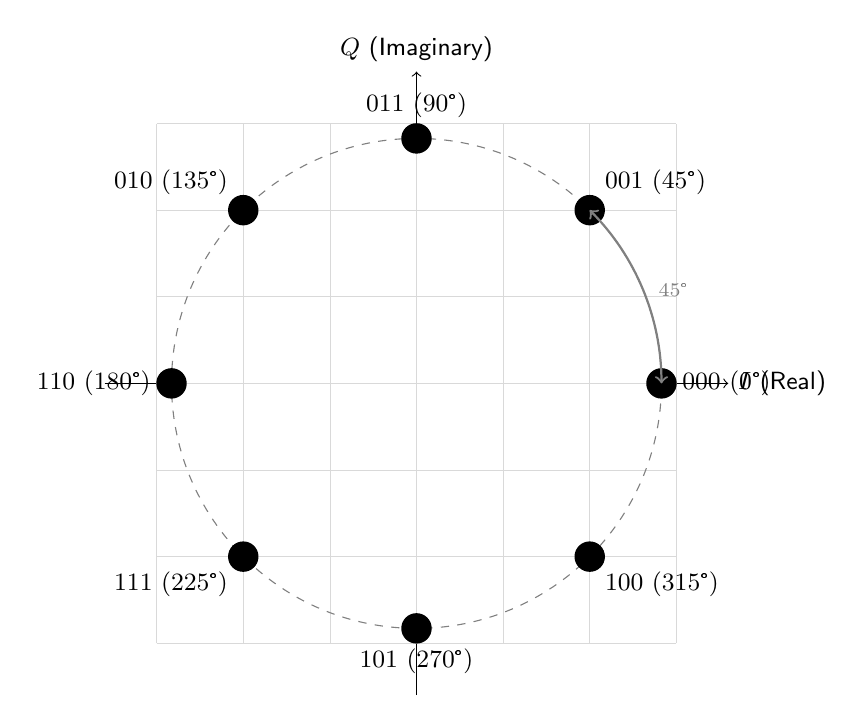
\begin{tikzpicture}[scale=2.2]
% Axes
\draw[->] (-1.8,0) -- (1.8,0) node[right] {\sffamily\small $I$ (Real)};
\draw[->] (0,-1.8) -- (0,1.8) node[above] {\sffamily\small $Q$ (Imaginary)};

% Grid
\draw[very thin,gray!30] (-1.5,-1.5) grid[step=0.5] (1.5,1.5);

% Unit circle
\draw[dashed,gray] (0,0) circle (1.4142);

% Constellation points with Gray coding
\fill[black] (1.4142,0) circle (2.5pt) node[right=4pt,font=\small] {000 (0°)};
\fill[black] (1,1) circle (2.5pt) node[above right=2pt,font=\small] {001 (45°)};
\fill[black] (0,1.4142) circle (2.5pt) node[above=4pt,font=\small] {011 (90°)};
\fill[black] (-1,1) circle (2.5pt) node[above left=2pt,font=\small] {010 (135°)};
\fill[black] (-1.4142,0) circle (2.5pt) node[left=4pt,font=\small] {110 (180°)};
\fill[black] (-1,-1) circle (2.5pt) node[below left=2pt,font=\small] {111 (225°)};
\fill[black] (0,-1.4142) circle (2.5pt) node[below=4pt,font=\small] {101 (270°)};
\fill[black] (1,-1) circle (2.5pt) node[below right=2pt,font=\small] {100 (315°)};

% Angular spacing annotation
\draw[<->,thick,gray] (1.4142,0) arc (0:45:1.4142) node[midway,right=2pt,font=\scriptsize] {45°};
\end{tikzpicture}
\end{center}

This maximum Euclidean distance constellation on the unit circle maintains constant envelope ($|s_m| = A$ for all $m$), enabling operation with nonlinear power amplifiers at saturation.

\subsection{Gray Coding}

Adjacent constellation points differ by only one bit (Gray coding) to minimize bit errors when symbol errors occur:

\begin{center}
\begin{tabular}{@{}ccccc@{}}
\toprule
Symbol & Gray Code & Phase & $I_m/A$ & $Q_m/A$ \\
\midrule
0 & 000 & $0°$ & 1.000 & 0.000 \\
1 & 001 & $45°$ & 0.707 & 0.707 \\
2 & 011 & $90°$ & 0.000 & 1.000 \\
3 & 010 & $135°$ & $-0.707$ & 0.707 \\
4 & 110 & $180°$ & $-1.000$ & 0.000 \\
5 & 111 & $225°$ & $-0.707$ & $-0.707$ \\
6 & 101 & $270°$ & 0.000 & $-1.000$ \\
7 & 100 & $315°$ & 0.707 & $-0.707$ \\
\bottomrule
\end{tabular}
\end{center}

Note that adjacent symbols (e.g., 000 $\rightarrow$ 001 $\rightarrow$ 011) differ by exactly one bit, minimizing the number of bit errors when noise causes a decision error to an adjacent symbol.

\section{Signal Characteristics}

\subsection{Constant Envelope Property}

All 8PSK symbols have identical amplitude:
\begin{equation}
|s_m| = A \quad \text{for all } m = 0, 1, \ldots, 7
\end{equation}

This constant envelope property provides a critical advantage:
\begin{itemize}
\item[\checkmark] Power amplifier can operate at saturation (maximum DC-to-RF efficiency)
\item[\checkmark] No amplitude modulation $\rightarrow$ no AM-PM distortion
\item[\checkmark] Peak-to-Average Power Ratio (PAPR) = 0~dB
\item[\checkmark] Compatible with nonlinear satellite TWTAs
\end{itemize}

\subsection{Symbol and Bit Energy}

The energy per symbol (normalized to unit symbol period $T_s = 1$):
\begin{equation}
E_s = \int_0^{T_s} |s_m(t)|^2 \, dt = A^2 T_s = A^2
\end{equation}

Since 8PSK transmits 3 bits per symbol:
\begin{equation}
E_b = \frac{E_s}{\log_2(8)} = \frac{E_s}{3} = \frac{A^2}{3}
\end{equation}
where:
\begin{itemize}
\item $E_s$ = energy per symbol (joules)
\item $E_b$ = energy per bit (joules)
\end{itemize}

\subsection{Minimum Euclidean Distance}

The minimum distance between adjacent constellation points is critical for noise immunity:
\begin{equation}
d_{\min} = 2A\sin\left(\frac{\pi}{8}\right) = 2A \times 0.3827 = 0.765A
\end{equation}

For normalized amplitude ($A = 1$): $d_{\min} = 0.765$

\textbf{Comparison with QPSK:}
\begin{itemize}
\item QPSK: $d_{\min} = \sqrt{2}A = 1.414A$ (at same average energy)
\item 8PSK: $d_{\min} = 0.765A$
\item \textbf{Ratio:} 8PSK minimum distance is $1.414/0.765 = 1.85\times$ smaller (5.3~dB)
\end{itemize}

This reduced separation explains why 8PSK requires approximately 3.5~dB higher SNR than QPSK to achieve the same BER.

\section{Modulation and Demodulation}

\subsection{Transmitter (IQ Modulator)}

The 8PSK modulator generates I and Q baseband components, then mixes with carrier quadrature signals:

\begin{center}
\begin{tikzpicture}[
  block/.style={rectangle, draw, minimum width=2.2cm, minimum height=1cm, font=\sffamily\small},
  node distance=2.2cm,
  font=\small
]
\node (input) {\sffamily Data\\3~bits};
\node[block, right of=input, node distance=2.8cm] (mapper) {Symbol\\Mapper};
\node[block, above right of=mapper, node distance=2.8cm, yshift=0.5cm] (i_filter) {RRC\\Filter};
\node[block, below right of=mapper, node distance=2.8cm, yshift=-0.5cm] (q_filter) {RRC\\Filter};
\node[block, right of=i_filter, node distance=3cm] (i_mult) {Mixer\\$\times$};
\node[block, right of=q_filter, node distance=3cm] (q_mult) {Mixer\\$\times$};
\node[circle, draw, right of=i_mult, node distance=2.5cm, minimum size=0.8cm] (sum) {$+$};
\node[right of=sum, node distance=2.2cm] (output) {\sffamily 8PSK\\Output};

\node[below of=i_mult, node distance=1.5cm, font=\scriptsize] (cos) {$\cos(2\pi f_c t)$};
\node[below of=q_mult, node distance=1.5cm, font=\scriptsize] (sin) {$-\sin(2\pi f_c t)$};

\draw[->,thick] (input) -- (mapper);
\draw[->,thick] (mapper) -- node[above left,font=\scriptsize] {$I_m$} (i_filter);
\draw[->,thick] (mapper) -- node[below left,font=\scriptsize] {$Q_m$} (q_filter);
\draw[->,thick] (i_filter) -- (i_mult);
\draw[->,thick] (q_filter) -- (q_mult);
\draw[->,thick] (cos) -- (i_mult);
\draw[->,thick] (sin) -- (q_mult);
\draw[->,thick] (i_mult) -- (sum);
\draw[->,thick] (q_mult) -- (sum);
\draw[->,thick] (sum) -- (output);
\end{tikzpicture}
\end{center}

\textbf{Process:}
\begin{enumerate}
\item \textbf{Symbol mapping:} Map 3-bit groups to I/Q coordinates using Gray coding
\item \textbf{Pulse shaping:} Apply root raised-cosine (RRC) filter to limit bandwidth
\item \textbf{Upconversion:} Mix I with $\cos(2\pi f_c t)$ and Q with $-\sin(2\pi f_c t)$
\item \textbf{Combine:} Sum I and Q paths to generate RF signal
\end{enumerate}

The transmitted signal is:
\begin{equation}
s_{\text{RF}}(t) = I_m(t) \cos(2\pi f_c t) - Q_m(t) \sin(2\pi f_c t)
\end{equation}
where $I_m(t)$ and $Q_m(t)$ are the pulse-shaped baseband waveforms.

\subsection{Receiver (Coherent Detector)}

\begin{center}
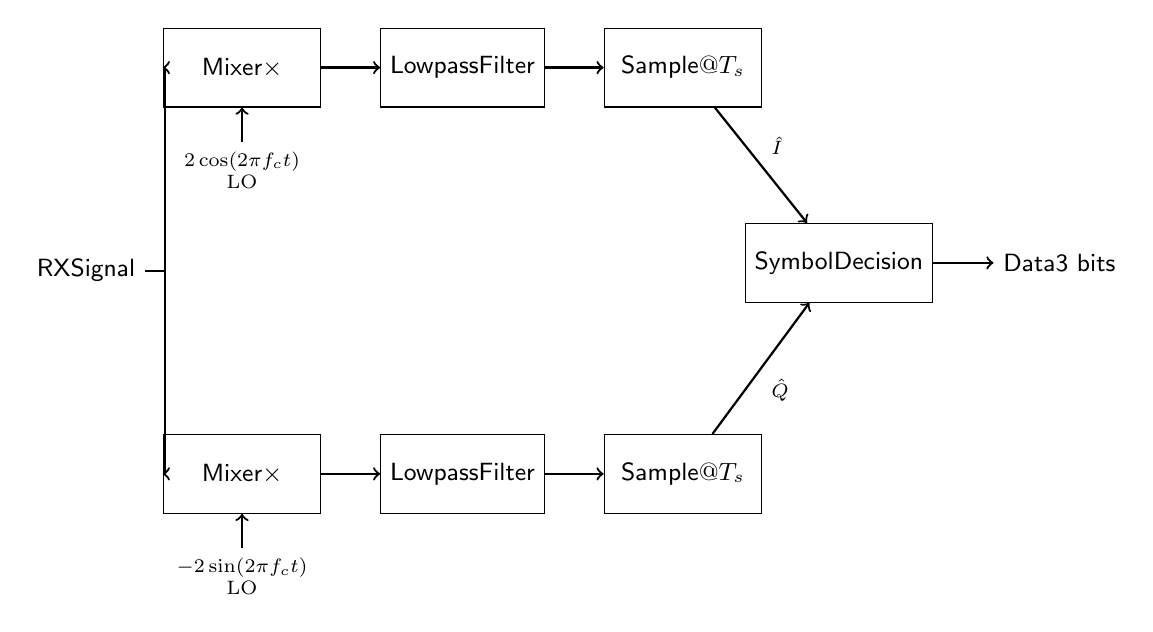
\begin{tikzpicture}[
  block/.style={rectangle, draw, minimum width=2cm, minimum height=1cm, font=\sffamily\small},
  node distance=2cm,
  font=\small
]
\node (input) {\sffamily RX\\Signal};
\node[block, above right of=input, node distance=2.8cm, yshift=0.6cm] (i_mult) {Mixer\\$\times$};
\node[block, below right of=input, node distance=2.8cm, yshift=-0.6cm] (q_mult) {Mixer\\$\times$};
\node[block, right of=i_mult, node distance=2.8cm] (i_lpf) {Lowpass\\Filter};
\node[block, right of=q_mult, node distance=2.8cm] (q_lpf) {Lowpass\\Filter};
\node[block, right of=i_lpf, node distance=2.8cm] (i_sample) {Sample\\$@T_s$};
\node[block, right of=q_lpf, node distance=2.8cm] (q_sample) {Sample\\$@T_s$};
\node[block, below right of=i_sample, node distance=2.8cm, yshift=-0.5cm] (decision) {Symbol\\Decision};
\node[right of=decision, node distance=2.8cm] (output) {\sffamily Data\\3~bits};

\node[below of=i_mult, node distance=1.3cm, font=\scriptsize, align=center] (lo_i) {$2\cos(2\pi f_c t)$\\LO};
\node[below of=q_mult, node distance=1.3cm, font=\scriptsize, align=center] (lo_q) {$-2\sin(2\pi f_c t)$\\LO};

\draw[->,thick] (input) -- ++(1,0) |- (i_mult);
\draw[->,thick] (input) -- ++(1,0) |- (q_mult);
\draw[->,thick] (lo_i) -- (i_mult);
\draw[->,thick] (lo_q) -- (q_mult);
\draw[->,thick] (i_mult) -- (i_lpf);
\draw[->,thick] (q_mult) -- (q_lpf);
\draw[->,thick] (i_lpf) -- (i_sample);
\draw[->,thick] (q_lpf) -- (q_sample);
\draw[->,thick] (i_sample) -- node[above right,font=\scriptsize] {$\hat{I}$} (decision);
\draw[->,thick] (q_sample) -- node[below right,font=\scriptsize] {$\hat{Q}$} (decision);
\draw[->,thick] (decision) -- (output);
\end{tikzpicture}
\end{center}

\begin{warningbox}
\textbf{Phase synchronization is critical.} The local oscillator must be exactly in phase with the transmitter carrier. A phase offset $\phi_e$ rotates the entire constellation, degrading performance. At $\phi_e = 22.5°$ (midpoint between symbols), complete decision ambiguity occurs.
\end{warningbox}

\textbf{Detection process:}
\begin{enumerate}
\item \textbf{Downconvert:} Mix received signal with local I/Q carriers
\item \textbf{Lowpass filter:} Remove $2f_c$ component, retain baseband
\item \textbf{Sample:} Capture I and Q values at optimal sampling instant
\item \textbf{Decision:} Find closest of 8 constellation points
\end{enumerate}

\textbf{Decision rule:} Calculate phase angle and quantize:
\begin{equation}
\hat{\phi} = \arctan\left(\frac{\hat{Q}}{\hat{I}}\right)
\end{equation}
\begin{equation}
\hat{m} = \left\lfloor \frac{\hat{\phi} + \pi/8}{2\pi/8} \right\rfloor \bmod 8
\end{equation}

The decision regions are 8 pie-slice wedges, each spanning $45°$ ($\pi/4$ radians), centered on each constellation point.

\subsection{Differential 8PSK (D8PSK)}

Differential encoding avoids the carrier phase ambiguity inherent in coherent PSK systems.

\textbf{Encoding:} Data is encoded in the \emph{phase change} between consecutive symbols:
\begin{equation}
\phi_k = \phi_{k-1} + \Delta\phi_k \bmod 2\pi
\end{equation}
where $\Delta\phi_k \in \{0, \pi/4, \pi/2, 3\pi/4, \pi, 5\pi/4, 3\pi/2, 7\pi/4\}$ encodes 3 data bits.

\textbf{Demodulation:} Compute phase difference between consecutive received symbols:
\begin{equation}
\Delta\hat{\phi}_k = \hat{\phi}_k - \hat{\phi}_{k-1}
\end{equation}

The 3-bit data word is decoded from $\Delta\hat{\phi}_k$ rather than from the absolute phase $\hat{\phi}_k$.

\textbf{Trade-off:}
\begin{itemize}
\item[\checkmark] No carrier phase recovery needed (only frequency synchronization)
\item[\checkmark] Simpler receiver implementation
\item[\checkmark] Immune to 8-fold phase ambiguity
\item[\texttimes] Approximately 3~dB performance penalty versus coherent detection
\item[\texttimes] Error propagation (one symbol error affects two decoded symbols)
\end{itemize}

\section{Bit Error Rate (BER) Performance}

\subsection{Symbol Error Rate in AWGN}

For 8PSK in additive white Gaussian noise (AWGN) with coherent detection (high SNR approximation):
\begin{equation}
P_s \approx 2Q\left(\sqrt{\frac{2E_s}{N_0}} \sin\left(\frac{\pi}{8}\right)\right) = 2Q\left(0.765\sqrt{\frac{E_s}{N_0}}\right)
\end{equation}
where:
\begin{itemize}
\item $P_s$ = symbol error probability
\item $E_s$ = energy per symbol (joules)
\item $N_0$ = noise power spectral density (W/Hz)
\item $Q(x) = \frac{1}{\sqrt{2\pi}} \int_x^\infty e^{-t^2/2} \, dt$ (Gaussian Q-function)
\end{itemize}

\subsection{Bit Error Rate with Gray Coding}

With Gray coding, most symbol errors cause only a single bit error:
\begin{equation}
\mathrm{BER} \approx \frac{P_s}{\log_2(8)} = \frac{P_s}{3}
\end{equation}

Expressing BER in terms of $E_b/N_0$ using $E_s = 3E_b$:
\begin{equation}
\mathrm{BER} \approx \frac{2}{3}Q\left(0.765\sqrt{\frac{3E_b}{N_0}}\right) = \frac{2}{3}Q\left(1.325\sqrt{\frac{E_b}{N_0}}\right)
\end{equation}

\subsection{Required $E_b/N_0$ for Target BER}

To achieve BER $= 10^{-6}$:

\begin{center}
\begin{tabular}{@{}lcc@{}}
\toprule
Modulation & Required $E_b/N_0$ (dB) & Penalty vs BPSK \\
\midrule
BPSK & 10.5 & --- \\
QPSK & 10.5 & 0~dB \\
\textbf{8PSK} & \textbf{14.0} & \textbf{+3.5~dB} \\
16-PSK & 18.0 & +7.5~dB \\
32-PSK & 22.0 & +11.5~dB \\
\bottomrule
\end{tabular}
\end{center}

\textbf{Key observation:} Each doubling of $M$ (from $M$-PSK to $2M$-PSK) adds approximately 3.5--4~dB SNR requirement, making higher-order PSK increasingly impractical.

\subsection{BER Performance Comparison}

\begin{center}
\begin{tabular}{@{}ccccc@{}}
\toprule
$E_b/N_0$ (dB) & BPSK & QPSK & 8PSK & 16-PSK \\
\midrule
6 & $1.9 \times 10^{-3}$ & $1.9 \times 10^{-3}$ & $4.0 \times 10^{-2}$ & $1.5 \times 10^{-1}$ \\
8 & $5.6 \times 10^{-5}$ & $5.6 \times 10^{-5}$ & $8.0 \times 10^{-3}$ & $8.0 \times 10^{-2}$ \\
10 & $3.9 \times 10^{-6}$ & $3.9 \times 10^{-6}$ & $7.0 \times 10^{-4}$ & $3.0 \times 10^{-2}$ \\
12 & $7.8 \times 10^{-8}$ & $7.8 \times 10^{-8}$ & $4.0 \times 10^{-5}$ & $8.0 \times 10^{-3}$ \\
14 & $7.7 \times 10^{-10}$ & $7.7 \times 10^{-10}$ & $1.0 \times 10^{-6}$ & $7.0 \times 10^{-4}$ \\
\bottomrule
\end{tabular}
\end{center}

\textbf{Key observation:} At a given SNR, higher-order PSK schemes suffer significantly higher BER due to reduced minimum distance between constellation points. To maintain the same BER as lower-order schemes, higher SNR is required.

\section{Bandwidth Efficiency}

The symbol rate for $M$-ary modulation is:
\begin{equation}
R_s = \frac{R_b}{\log_2(M)} \quad \text{(symbols/second)}
\end{equation}
where $R_b$ is the bit rate (bps).

With raised-cosine pulse shaping (roll-off factor $\alpha$), the occupied bandwidth is:
\begin{equation}
B = (1 + \alpha) R_s = (1 + \alpha) \frac{R_b}{\log_2(M)} \quad \text{(Hz)}
\end{equation}

The spectral efficiency (data rate per unit bandwidth) is:
\begin{equation}
\eta = \frac{R_b}{B} = \frac{\log_2(M)}{1 + \alpha} \quad \text{(bps/Hz)}
\end{equation}

\subsection{Comparison of PSK Schemes}

For $\alpha = 0.35$ (typical raised-cosine roll-off):

\begin{center}
\begin{tabular}{@{}lcccc@{}}
\toprule
Modulation & Bits/Symbol & $\eta$ (bps/Hz) & Required $E_b/N_0$ & Relative SNR \\
\midrule
BPSK & 1 & 0.74 & 10.5~dB & Baseline \\
QPSK & 2 & 1.48 & 10.5~dB & 0~dB \\
\textbf{8PSK} & \textbf{3} & \textbf{2.22} & \textbf{14.0~dB} & \textbf{+3.5~dB} \\
16-PSK & 4 & 2.96 & 18.0~dB & +7.5~dB \\
32-PSK & 5 & 3.70 & 22.0~dB & +11.5~dB \\
\bottomrule
\end{tabular}
\end{center}

\begin{calloutbox}{Spectral Efficiency vs Power Efficiency Trade-off}
8PSK provides 50\% higher spectral efficiency than QPSK (2.22 vs 1.48~bps/Hz) but requires 3.5~dB more SNR to achieve the same BER. This makes 8PSK ideal for bandwidth-limited systems with adequate link margin, such as:
\begin{itemize}
\item Satellite broadcasting (DVB-S2)
\item Microwave backhaul links
\item High-throughput military SATCOM
\end{itemize}
\end{calloutbox}

\subsection{Higher-Order PSK}\label{higher-order-psk}

\subsubsection{16-PSK}\label{psk}

\textbf{16 phase states}: 22.5\$\^{}\textbackslash circ\$ spacing

\textbf{Bits per symbol}: 4

\textbf{Minimum distance}: \(d_{\min} = 2A\sin(\pi/16) = 0.39A\)

\textbf{Performance}: \textasciitilde4 dB worse than 8PSK (at same BER)

\textbf{Problem}: Very sensitive to phase noise (small angular
separation)

\begin{center}\rule{0.5\linewidth}{0.5pt}\end{center}

\subsubsection{32-PSK and Beyond}\label{psk-and-beyond}

\textbf{32-PSK}: 11.25\$\^{}\textbackslash circ\$ spacing, 5 bits/symbol

\textbf{64-PSK}: 5.625\$\^{}\textbackslash circ\$ spacing, 6 bits/symbol

\textbf{Practical limit}: M \textgreater{} 16 rarely used - Phase noise
becomes limiting factor - QAM more efficient for M \textgreater{} 8

\begin{center}\rule{0.5\linewidth}{0.5pt}\end{center}

\subsection{8PSK vs Other Modulations}\label{psk-vs-other-modulations}

\subsubsection{8PSK vs 16-QAM}\label{psk-vs-16-qam}

\textbf{Same spectral efficiency} (\$\textbackslash approx\$2.2
bits/sec/Hz with \$\textbackslash alpha\$=0.35): - \textbf{8PSK}: 3
bits/symbol - \textbf{16-QAM}: 4 bits/symbol @
1.33\$\textbackslash times\$ symbol rate

\textbf{BER comparison} @ BER =
10\textbackslash textsuperscript\{-\}\textbackslash textsuperscript\{6\}:
- \textbf{8PSK}: 14 dB Eb/N0 - \textbf{16-QAM}: 14.5 dB Eb/N0

\textbf{Advantage 8PSK}: Constant envelope (PA efficiency)

\textbf{Advantage 16-QAM}: Slightly better BER, more flexible coding
rates

\begin{center}\rule{0.5\linewidth}{0.5pt}\end{center}

\subsubsection{8PSK vs OFDM with QPSK}\label{psk-vs-ofdm-with-qpsk}

\textbf{Wideband system} (20 MHz):

\textbf{8PSK single carrier}: - 6.67 Msps, 20 Mbps - Requires
equalization (frequency-selective fading) - Constant envelope

\textbf{OFDM with QPSK} (64 subcarriers): - 312.5 kHz per subcarrier
(flat fading) - 20 Mbps total - Varying envelope (PAPR \textasciitilde10
dB)

\textbf{Trade-off}: OFDM handles multipath better, 8PSK more
PA-efficient

\begin{center}\rule{0.5\linewidth}{0.5pt}\end{center}

\subsection{Phase Noise Sensitivity}\label{phase-noise-sensitivity}

\textbf{Oscillator phase noise} \(\phi_n(t)\) rotates constellation:

\[
r_m(t) = A e^{j(\phi_m + \phi_n(t))} + n(t)
\]

\textbf{Phase error} \(\phi_n\) causes: - \textbf{Rotation}: All symbols
rotate equally - \textbf{Spreading}: Random jitter
\$\textbackslash rightarrow\$ Constellation blur

\textbf{Sensitivity} (angular spacing): - \textbf{QPSK}:
90\$\^{}\textbackslash circ\$ spacing (robust) - \textbf{8PSK}:
45\$\^{}\textbackslash circ\$ spacing (moderate) - \textbf{16-PSK}:
22.5\$\^{}\textbackslash circ\$ spacing (sensitive) - \textbf{32-PSK}:
11.25\$\^{}\textbackslash circ\$ spacing (very sensitive)

\textbf{Rule of thumb}: Phase noise RMS should be \textless{} 1/10 of
angular spacing

\textbf{Example}: 8PSK with 45\$\^{}\textbackslash circ\$ spacing -
Tolerable phase noise: \textasciitilde4.5\$\^{}\textbackslash circ\$ RMS
- Equivalent phase noise: \textasciitilde-25 dBc integrated (tight
spec!)

\begin{center}\rule{0.5\linewidth}{0.5pt}\end{center}

\subsection{Practical Implementations}\label{practical-implementations}

\subsubsection{1. DVB-S2 (Satellite TV)}\label{dvb-s2-satellite-tv}

\textbf{8PSK} used for high data rates: - \textbf{QPSK}: Low C/N (rain
fade conditions) - \textbf{8PSK}: Clear sky, high throughput -
\textbf{Adaptive Coding \& Modulation (ACM)}: Switch based on link
quality

\textbf{Example}: - QPSK 1/2: 1 bit/symbol effective
\$\textbackslash rightarrow\$ 0.74 bits/sec/Hz - 8PSK 3/4: 2.25
bits/symbol effective \$\textbackslash rightarrow\$ 1.67 bits/sec/Hz -
\textbf{2.25\$\textbackslash times\$ throughput} when SNR permits

\begin{center}\rule{0.5\linewidth}{0.5pt}\end{center}

\subsubsection{2. Military SATCOM
(MILSTAR)}\label{military-satcom-milstar}

\textbf{Differential 8PSK}: - Robust against jamming -
Low-probability-of-intercept (LPI) - Spread spectrum combined with D8PSK

\begin{center}\rule{0.5\linewidth}{0.5pt}\end{center}

\subsubsection{3. Microwave Backhaul}\label{microwave-backhaul}

\textbf{Point-to-point links} (cellular backhaul): - \textbf{Clear
weather}: 256-QAM (8 bits/symbol) - \textbf{Rain fade}: Adaptive down to
8PSK or QPSK - \textbf{Example}: 6-11 GHz bands, 28/56 MHz channels

\begin{center}\rule{0.5\linewidth}{0.5pt}\end{center}

\subsubsection{4. Deep Space
Communications}\label{deep-space-communications}

\textbf{NASA/ESA}: Primarily BPSK/QPSK (maximize link margin)

\textbf{Emerging}: 8PSK for high-rate science data return - \textbf{Mars
orbiters}: 8PSK @ Ka-band (32 GHz) - \textbf{Trade-off}:
3\$\textbackslash times\$ data rate vs 3.5 dB link margin

\begin{center}\rule{0.5\linewidth}{0.5pt}\end{center}

\subsection{Implementation Challenges}\label{implementation-challenges}

\subsubsection{1. Carrier Phase Recovery}\label{carrier-phase-recovery}

\textbf{8PSK phase ambiguity}: 8-fold (every
45\$\^{}\textbackslash circ\$)

\textbf{Pilot-aided sync}: - Insert known pilot symbols - Estimate phase
offset - Correct data symbols

\textbf{Blind sync}: - 8th-power loop (remove modulation) - Costas loop
(feedback) - Decision-directed (after initial acquisition)

\textbf{See}: {[}{[}Synchronization-(Carrier,-Timing,-Frame){]}{]}

\begin{center}\rule{0.5\linewidth}{0.5pt}\end{center}

\subsubsection{2. Timing Recovery}\label{timing-recovery}

\textbf{Symbol clock} must be accurate:

\textbf{Timing jitter} causes: - Sampling offset
\$\textbackslash rightarrow\$ ISI - Increased BER

\textbf{Early-late gate} detector: - Sample early, on-time, late -
Adjust clock based on correlation

\begin{center}\rule{0.5\linewidth}{0.5pt}\end{center}

\subsubsection{3. Nonlinear PA
Distortion}\label{nonlinear-pa-distortion}

\textbf{8PSK constant envelope}: Tolerates PA saturation

\textbf{BUT}: Pulse shaping filter creates envelope variations - Raised
cosine filter \$\textbackslash rightarrow\$ 3-4 dB PAPR - PA must back
off \$\textbackslash rightarrow\$ Reduced efficiency

\textbf{Mitigation}: - \textbf{Constant envelope pulse shaping}: MSK,
GMSK (no overshoot) - \textbf{Predistortion}: Digital or analog
linearization

\begin{center}\rule{0.5\linewidth}{0.5pt}\end{center}

\subsubsection{4. Frequency Offset}\label{frequency-offset}

\textbf{Carrier frequency offset} \(\Delta f\) rotates constellation:

\[
r(t) = s(t) e^{j2\pi \Delta f t}
\]

\textbf{Tolerable offset} (rule of thumb):
\(|\Delta f| < 0.01 \times R_s\)

\textbf{Example}: 8PSK @ 1 Msps - Tolerable offset: \textless{} 10 kHz -
Oscillator spec: \textless{} 10 ppm @ 1 GHz carrier (= 10 kHz)

\begin{center}\rule{0.5\linewidth}{0.5pt}\end{center}

\subsection{Adaptive Modulation \& Coding
(AMC)}\label{adaptive-modulation-coding-amc}

\textbf{Dynamically select modulation} based on channel quality:

\textbf{Link adaptation table}:

{\def\LTcaptype{} % do not increment counter
\begin{longtable}[]{@{}lllll@{}}
\toprule\noalign{}
C/N (dB) & Modulation & Code Rate & Spectral Eff. & Target BER \\
\midrule\noalign{}
\endhead
\bottomrule\noalign{}
\endlastfoot
2-5 & QPSK & 1/4 & 0.5 &
10\textbackslash textsuperscript\{-\}\textbackslash textsuperscript\{7\} \\
5-7 & QPSK & 1/2 & 1.0 &
10\textbackslash textsuperscript\{-\}\textbackslash textsuperscript\{7\} \\
7-9 & QPSK & 3/4 & 1.5 &
10\textbackslash textsuperscript\{-\}\textbackslash textsuperscript\{7\} \\
9-11 & 8PSK & 2/3 & 2.0 &
10\textbackslash textsuperscript\{-\}\textbackslash textsuperscript\{7\} \\
11-13 & 8PSK & 3/4 & 2.25 &
10\textbackslash textsuperscript\{-\}\textbackslash textsuperscript\{7\} \\
13-15 & 16-QAM & 2/3 & 2.67 &
10\textbackslash textsuperscript\{-\}\textbackslash textsuperscript\{7\} \\
\end{longtable}
}

\textbf{Benefit}: Maximize throughput while maintaining target BER

\begin{center}\rule{0.5\linewidth}{0.5pt}\end{center}

\subsection{Gray Coding}\label{gray-coding}

\textbf{Gray code}: Adjacent symbols differ by \textbf{1 bit}

\textbf{Benefit}: Symbol error \$\textbackslash rightarrow\$ Likely
1-bit error (not 2 or 3)

\textbf{8PSK Gray mapping}:

{\def\LTcaptype{} % do not increment counter
\begin{longtable}[]{@{}llll@{}}
\toprule\noalign{}
Symbol & Binary & Phase (\$\^{}\textbackslash circ\$) & Gray Code \\
\midrule\noalign{}
\endhead
\bottomrule\noalign{}
\endlastfoot
0 & 000 & 0 & 000 \\
1 & 001 & 45 & 001 \\
2 & 010 & 90 & 011 \\
3 & 011 & 135 & 010 \\
4 & 100 & 180 & 110 \\
5 & 101 & 225 & 111 \\
6 & 110 & 270 & 101 \\
7 & 111 & 315 & 100 \\
\end{longtable}
}

\textbf{Natural binary}: Symbol error \$\textbackslash rightarrow\$ Up
to 3-bit error

\textbf{Gray coding}: Symbol error \$\textbackslash rightarrow\$
Typically 1-bit error (maybe 2)

\textbf{BER improvement}: \textasciitilde2\$\textbackslash times\$
better with Gray coding

\begin{center}\rule{0.5\linewidth}{0.5pt}\end{center}

\subsection{Pulse Shaping}\label{pulse-shaping}

\textbf{Rectangular pulses}: Infinite bandwidth (sinc spectrum)

\textbf{Raised cosine} (RC):

\[
P(f) = \begin{cases}
T_s & |f| \leq \frac{1-\alpha}{2T_s} \\
\frac{T_s}{2}\left[1 + \cos\left(\frac{\pi T_s}{\alpha}\left[|f| - \frac{1-\alpha}{2T_s}\right]\right)\right] & \frac{1-\alpha}{2T_s} < |f| \leq \frac{1+\alpha}{2T_s} \\
0 & |f| > \frac{1+\alpha}{2T_s}
\end{cases}
\]

\textbf{Roll-off factor} \$\textbackslash alpha\$: -
\textbf{\$\textbackslash alpha\$ = 0}: Brick-wall (infinite time,
impractical) - \textbf{\$\textbackslash alpha\$ = 0.35}: Common (35\%
excess BW, moderate time decay) - \textbf{\$\textbackslash alpha\$ = 1}:
Gentle roll-off (100\% excess BW, fast time decay)

\textbf{Root raised cosine} (RRC): Split between TX and RX (matched
filter)

\begin{center}\rule{0.5\linewidth}{0.5pt}\end{center}

\subsection{Summary Table}\label{summary-table}

{\def\LTcaptype{} % do not increment counter
\begin{longtable}[]{@{}
  >{\raggedright\arraybackslash}p{(\linewidth - 12\tabcolsep) * \real{0.1395}}
  >{\raggedright\arraybackslash}p{(\linewidth - 12\tabcolsep) * \real{0.1163}}
  >{\raggedright\arraybackslash}p{(\linewidth - 12\tabcolsep) * \real{0.1628}}
  >{\raggedright\arraybackslash}p{(\linewidth - 12\tabcolsep) * \real{0.1628}}
  >{\raggedright\arraybackslash}p{(\linewidth - 12\tabcolsep) * \real{0.1744}}
  >{\raggedright\arraybackslash}p{(\linewidth - 12\tabcolsep) * \real{0.0698}}
  >{\raggedright\arraybackslash}p{(\linewidth - 12\tabcolsep) * \real{0.1744}}@{}}
\toprule\noalign{}
\begin{minipage}[b]{\linewidth}\raggedright
Modulation
\end{minipage} & \begin{minipage}[b]{\linewidth}\raggedright
Bits/sym
\end{minipage} & \begin{minipage}[b]{\linewidth}\raggedright
Min Distance
\end{minipage} & \begin{minipage}[b]{\linewidth}\raggedright
Eb/N0 (\(10^{-6}\))
\end{minipage} & \begin{minipage}[b]{\linewidth}\raggedright
Spectral Eff.
\end{minipage} & \begin{minipage}[b]{\linewidth}\raggedright
PAPR
\end{minipage} & \begin{minipage}[b]{\linewidth}\raggedright
Best Use Case
\end{minipage} \\
\midrule\noalign{}
\endhead
\bottomrule\noalign{}
\endlastfoot
\textbf{BPSK} & 1 & 2A & 10.5 dB & 0.74 & 0 dB & Deep space, long
range \\
\textbf{QPSK} & 2 & \$\textbackslash sqrt\{\}\$2 A & 10.5 dB & 1.48 & 0
dB & Balanced (most common) \\
\textbf{8PSK} & 3 & 0.765A & 14 dB & 2.22 & 0 dB & High throughput, PA
efficiency \\
\textbf{16-PSK} & 4 & 0.39A & 18 dB & 2.96 & 0 dB & Rarely (QAM
better) \\
\textbf{16-QAM} & 4 & 0.63A & 14.5 dB & 2.96 & 2.6 dB & High throughput
(non-const env) \\
\end{longtable}
}

\begin{center}\rule{0.5\linewidth}{0.5pt}\end{center}

\subsection{Related Topics}\label{related-topics}

\begin{itemize}
\tightlist
\item
  \textbf{{[}{[}QPSK-Modulation{]}{]}}: Lower-order PSK (2 bits/symbol)
\item
  \textbf{{[}{[}Binary-Phase-Shift-Keying-(BPSK){]}{]}}: Simplest PSK
\item
  \textbf{{[}{[}Constellation-Diagrams{]}{]}}: Visualizing PSK
\item
  \textbf{{[}{[}Bit-Error-Rate-(BER){]}{]}}: Performance metric
\item
  \textbf{{[}{[}Synchronization-(Carrier,-Timing,-Frame){]}{]}}: Carrier
  recovery for coherent detection
\item
  \textbf{{[}{[}OFDM-\&-Multicarrier-Modulation{]}{]}}: Uses QPSK/8PSK
  per subcarrier
\end{itemize}

\begin{center}\rule{0.5\linewidth}{0.5pt}\end{center}

\textbf{Key takeaway}: \textbf{8PSK transmits 3 bits/symbol using 8
phase states.} Constant envelope = PA efficient. 50\% more spectral
efficiency than QPSK but needs +3.5 dB SNR. Used in satellite (DVB-S2)
and backhaul. Higher-order PSK (16, 32, 64) rarely used due to phase
noise sensitivity-\/-\/-QAM preferred for M \textgreater{} 8. Gray
coding reduces BER by limiting bit errors per symbol error. Adaptive
modulation switches between QPSK/8PSK/16-QAM based on link quality.

\begin{center}\rule{0.5\linewidth}{0.5pt}\end{center}

\emph{This wiki is part of the {[}{[}Home\textbar Chimera Project{]}{]}
documentation.}
